\section{Interaction Patterns Between Ase1 and Dynamic Microtubules}
\label{sec:Ase1}

\subsection{The effect of Ase1 on microtubule dynamic instability}
\begin{figure}[h]
    \centering
    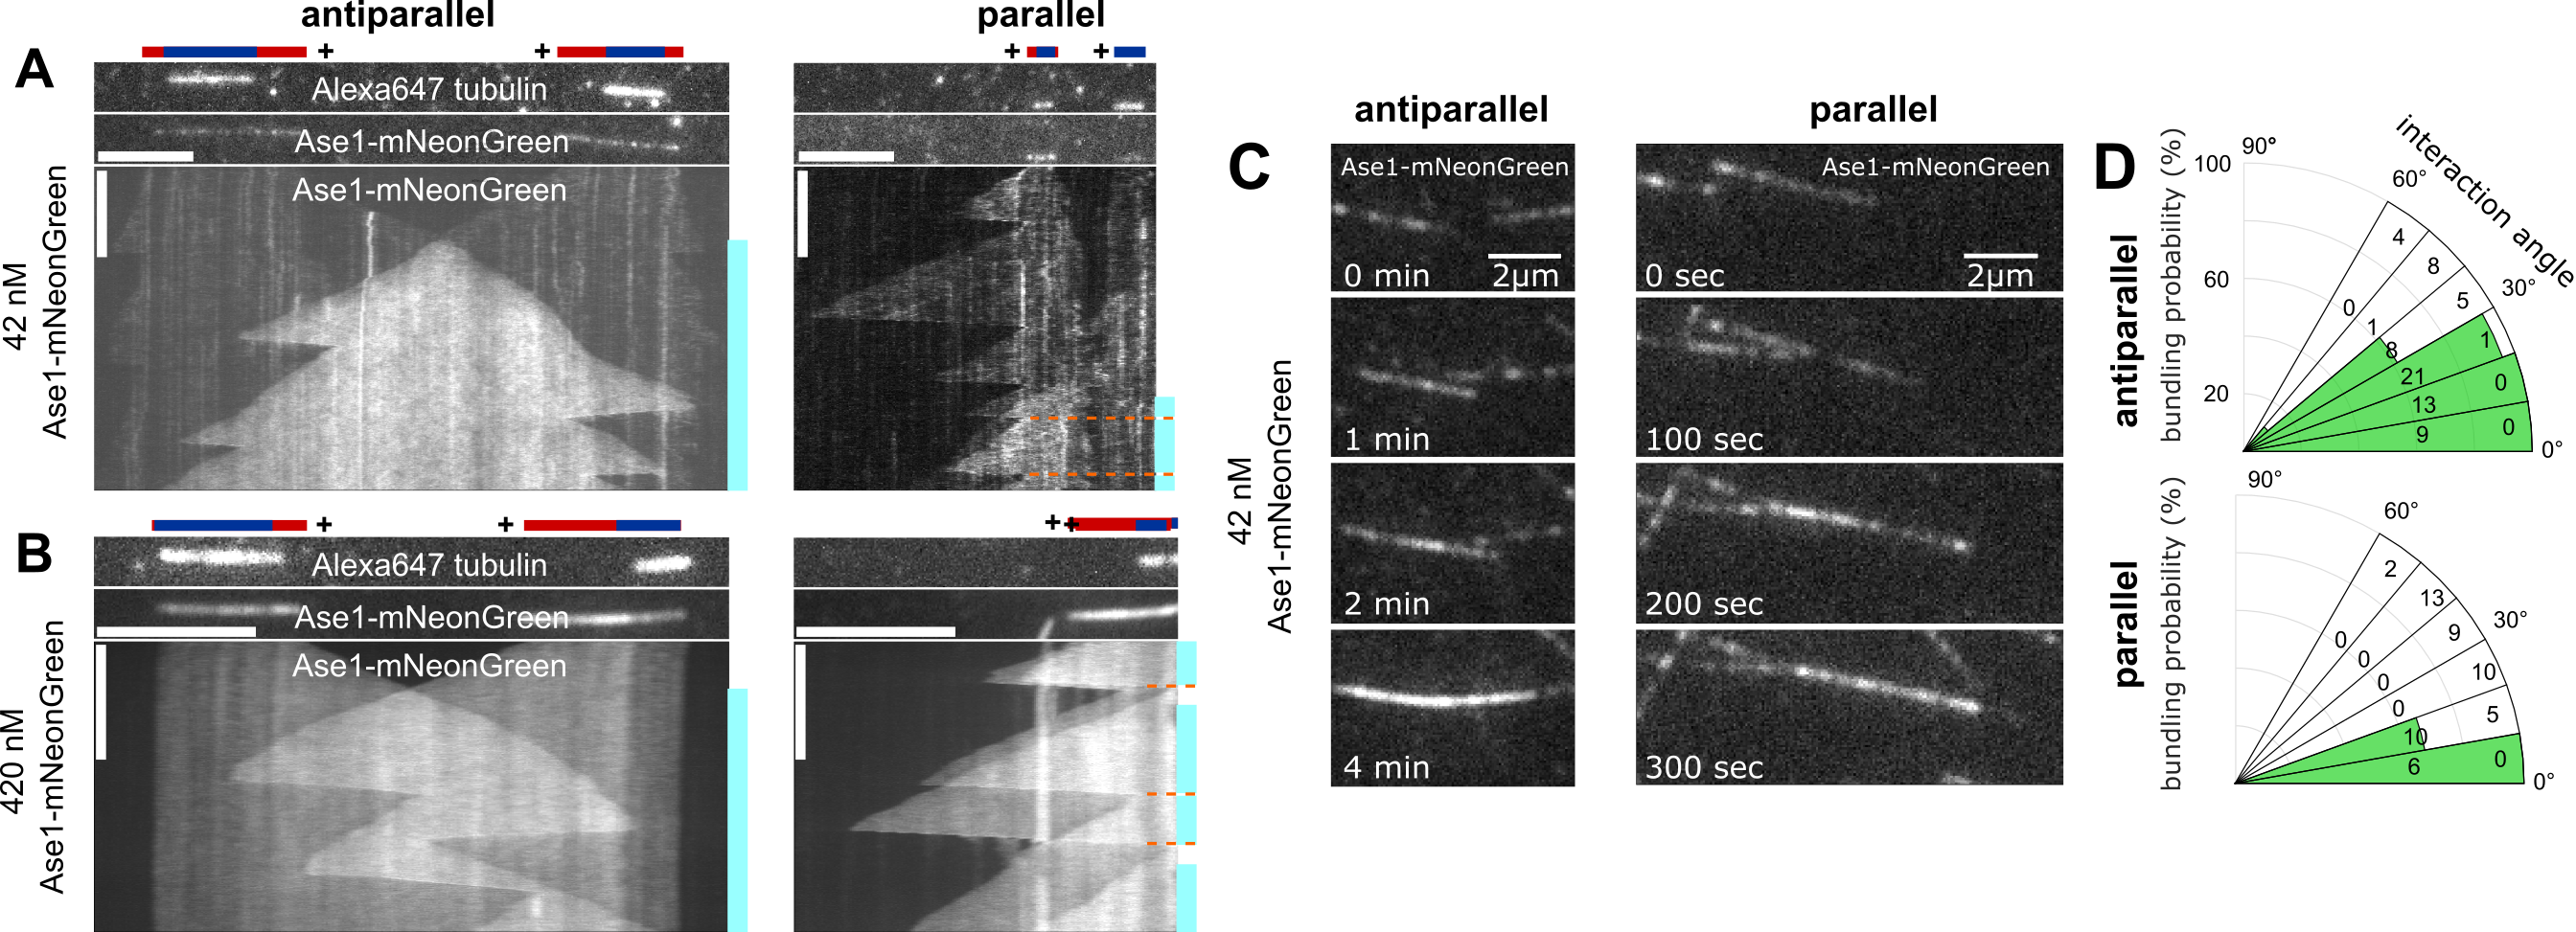
\includegraphics[width=1\linewidth]{Figures/ase1_1a.png}
    \caption[With dynamic microtubule extensions and Ase1, we observed microtubule bundling as previously reported.]{
    (A) Kymographs of an antiparallel (left panel) and a parallel microtubule overlap forming due to the microtubules polymerizing such to enable bundling by Ase1, which is present in solution (42nM). The scale bars are 5 micron and 10 minutes. In sketches, dynamic extensions with GDP lattices are red, and stabilized GMPCPP seeds are blue. The teal bars next to kymographs indicate the presence of regions of overlap (we only counted regions where the two partaking microtubule regions are constituted by GDP-tubulin, i.e., a seed stabilized by GMPCPP did not count). The orange lines indicate a termination of the overlapping period, as evaluated for \autoref{ase1b}A. (B) Same representation as A showing events from experiments performed at 420nM Ase1. (C) Snapshots of different events than shown in A and B, illustrating microtubule bundling (at 42nM). (D) Bundling probability for situations when microtubule plus ends encountered other microtubules, in either parallel or antiparallel orientation, versus the initial angle of interaction (results pooled for all Ase1-mNeonGreen concentrations). The outer numbers denote the numbers of recorded crossings at the respective angle, while the inner numbers denote the numbers of bundling events (the sum of both numbers is the total number of observed events). Panels taken from \cite{Krattenmacher2024}.
        }\label{ase1a}
\end{figure}
To investigate the interaction dynamics between diffusible microtubule crosslinkers and microtubules, we employed total internal reflection fluorescence (TIRF) and interference reflection microscopy (IRM) (\autoref{sec:microscopy}) time-lapse imaging of immobilized, GMPCPP-stabilized microtubule seeds in the presence of 30 µM free tubulin and varying concentrations of Ase1 (\autoref{methods}). At concentrations of 42 nM and 420 nM Ase1, we observed dynamic, Ase1-decorated microtubule extensions polymerizing from the microtubule seeds \pref{ase1a}{A,B}. When two microtubule plus ends, emanating from different seeds and polymerizing towards each other, encountered each other, the microtubules either bundled or crossed, depending on the angle of incidence. Typically, at high angles, the microtubules crossed and only interacted at the crossing point, while at small angles, either parallel or antiparallel associations could be formed \pref{ase1a}{C}. As previously reported \parencite{Janson2007}, antiparallel bundles formed even at large initial angles of incidence (up to 40°), while parallel bundles only formed at initial angles below 20° \pref{ase1a}{D}.\par
\begin{wrapfigure}{l}{0.4\textwidth}
    \centering
    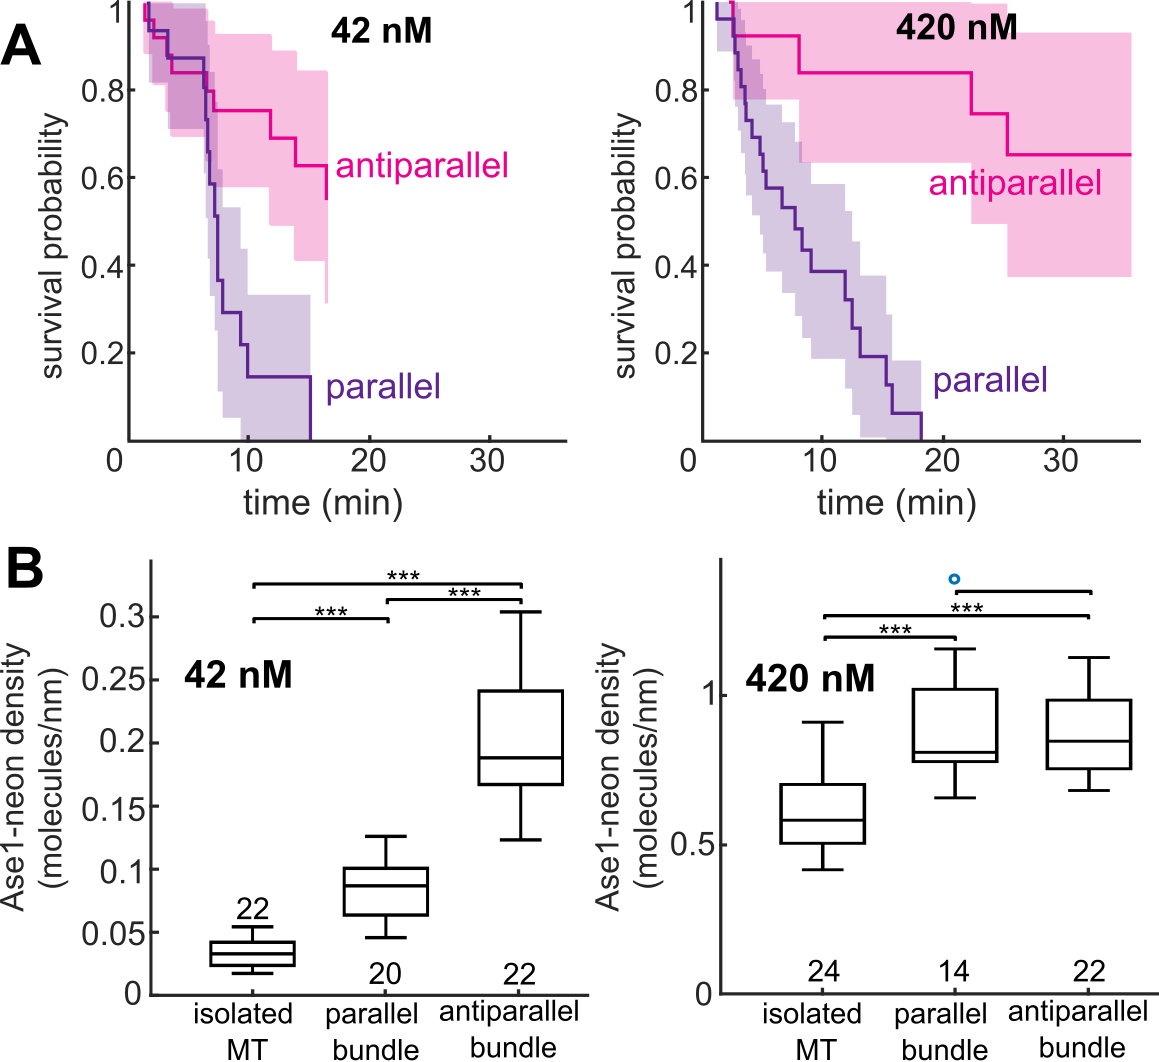
\includegraphics[width=1\linewidth]{Figures/ase1_1b.png}
    \caption[Ase1 selectively stabilizes antiparallel overlaps.]{
    (A) Survival probability of antiparallel and parallel overlaps, showing the probability that an overlap formed by two dynamic MT extensions persists at a given time after its formation (Methods). Semitransparent regions indicate 95\% lower and upper confidence bounds. (B) Quantification of the density of Ase1-mNeonGreen on isolated MTs and (anti)parallel bundles (Methods). The numbers below the boxes denote the number of analyzed microtubule bundles. Panels show data for MT plus ends (minus ends generally were not analyzed). Panels taken from \cite{Krattenmacher2024}.
        }\label{ase1b}
\end{wrapfigure}
Quantitative analysis revealed increased lifetimes of antiparallel overlaps compared to parallel ones\pref{ase1b}{A} Notably, at 42 nM Ase1 in solution, the Ase1 density on antiparallel overlaps was an order of magnitude higher than on parallel ones\pref{ase1b}{B} consistent with the previously reported differential affinities \parencite{Janson2007}. At 420 nM Ase1, we observed the density of Ase1 to be similar on antiparallel and parallel bundles, roughly twice the density found on isolated microtubules\pref{ase1b}{B} This possibly indicated that, at this high concentration, a similar number of Ase1 molecules was present within parallel and antiparallel overlaps. Note, however, that this value represents the total density of Ase1 at the bundle, which might differ from the density of Ase1 molecules directly engaged in MT crosslinking by being bound simultaneously to both microtubules. Despite similar decoration levels by Ase1, antiparallel overlaps were still significantly more stable than parallel ones\pref{ase1b}{A} Given the low polymerization velocity of minus ends, we very rarely observed antiparallel overlaps formed by two minus ends encountering each other, and we thus could not meaningfully quantify the associated lifetime. Generally, we chose to not analyze minus ends given that they are not dynamic \textit{in vivo} \parencite{dammer}.\par

To test whether the relative stability of antiparallel overlaps was caused by Ase1 crosslinking or the bundling itself (as was requested by a reviewer), we also conducted experiments at 10nM Ase1. At this concentration, we observed significantly less Ase1 within antiparallel bundles \pref{ase1c}{A}, and indeed, antiparallel bundles were no more stable than parallel bundles \pref{ase1c}{B}. Also, at 10nM Ase1 we observed antiparallel microtubules to no longer bundle as readily as at higher Ase1 concentrations \pref{ase1c}{C}. While we could detect an Ase1 signal at antiparallel overlaps, we did observe events where Ase1 crosslinking apparently was not strong enough to keep a MT plus end bundled to the MT along which it was growing in an antiparallel orientation \pref{ase1c}{D,E left panel}. Finally, to test whether microtubule bundling in our assays was partially a result of molecular crowding (and not Ase1), we performed an assay at 0nM Ase1. In absence of Ase1, microtubules never bundled, even when very close to each other over extended periods of time, indicating that molecular crowding did not play a role in the microtubule bundling we observed \pref{ase1c}{F}. \par

The relative stability of antiparallel overlaps at high Ase1 concentrations may at least partly owe to the fact that antiparallel overlaps grow with twice the speed of parallel overlaps (since both microtubules polymerize in opposite directions, however it should be noted that once a minus end has been surpassed the antiparallel overlaps does no longer grow as quickly on the side in question); hence, there is more opportunities for rescues to occur during depolymerization. However, our kymographs suggested that antiparallel overlaps may be additionally stabilized by an increase in rescue frequency \pref{ase1d}{A}, and we set out to quantify this issue next. \par

\begin{figure}[h]
    \centering
    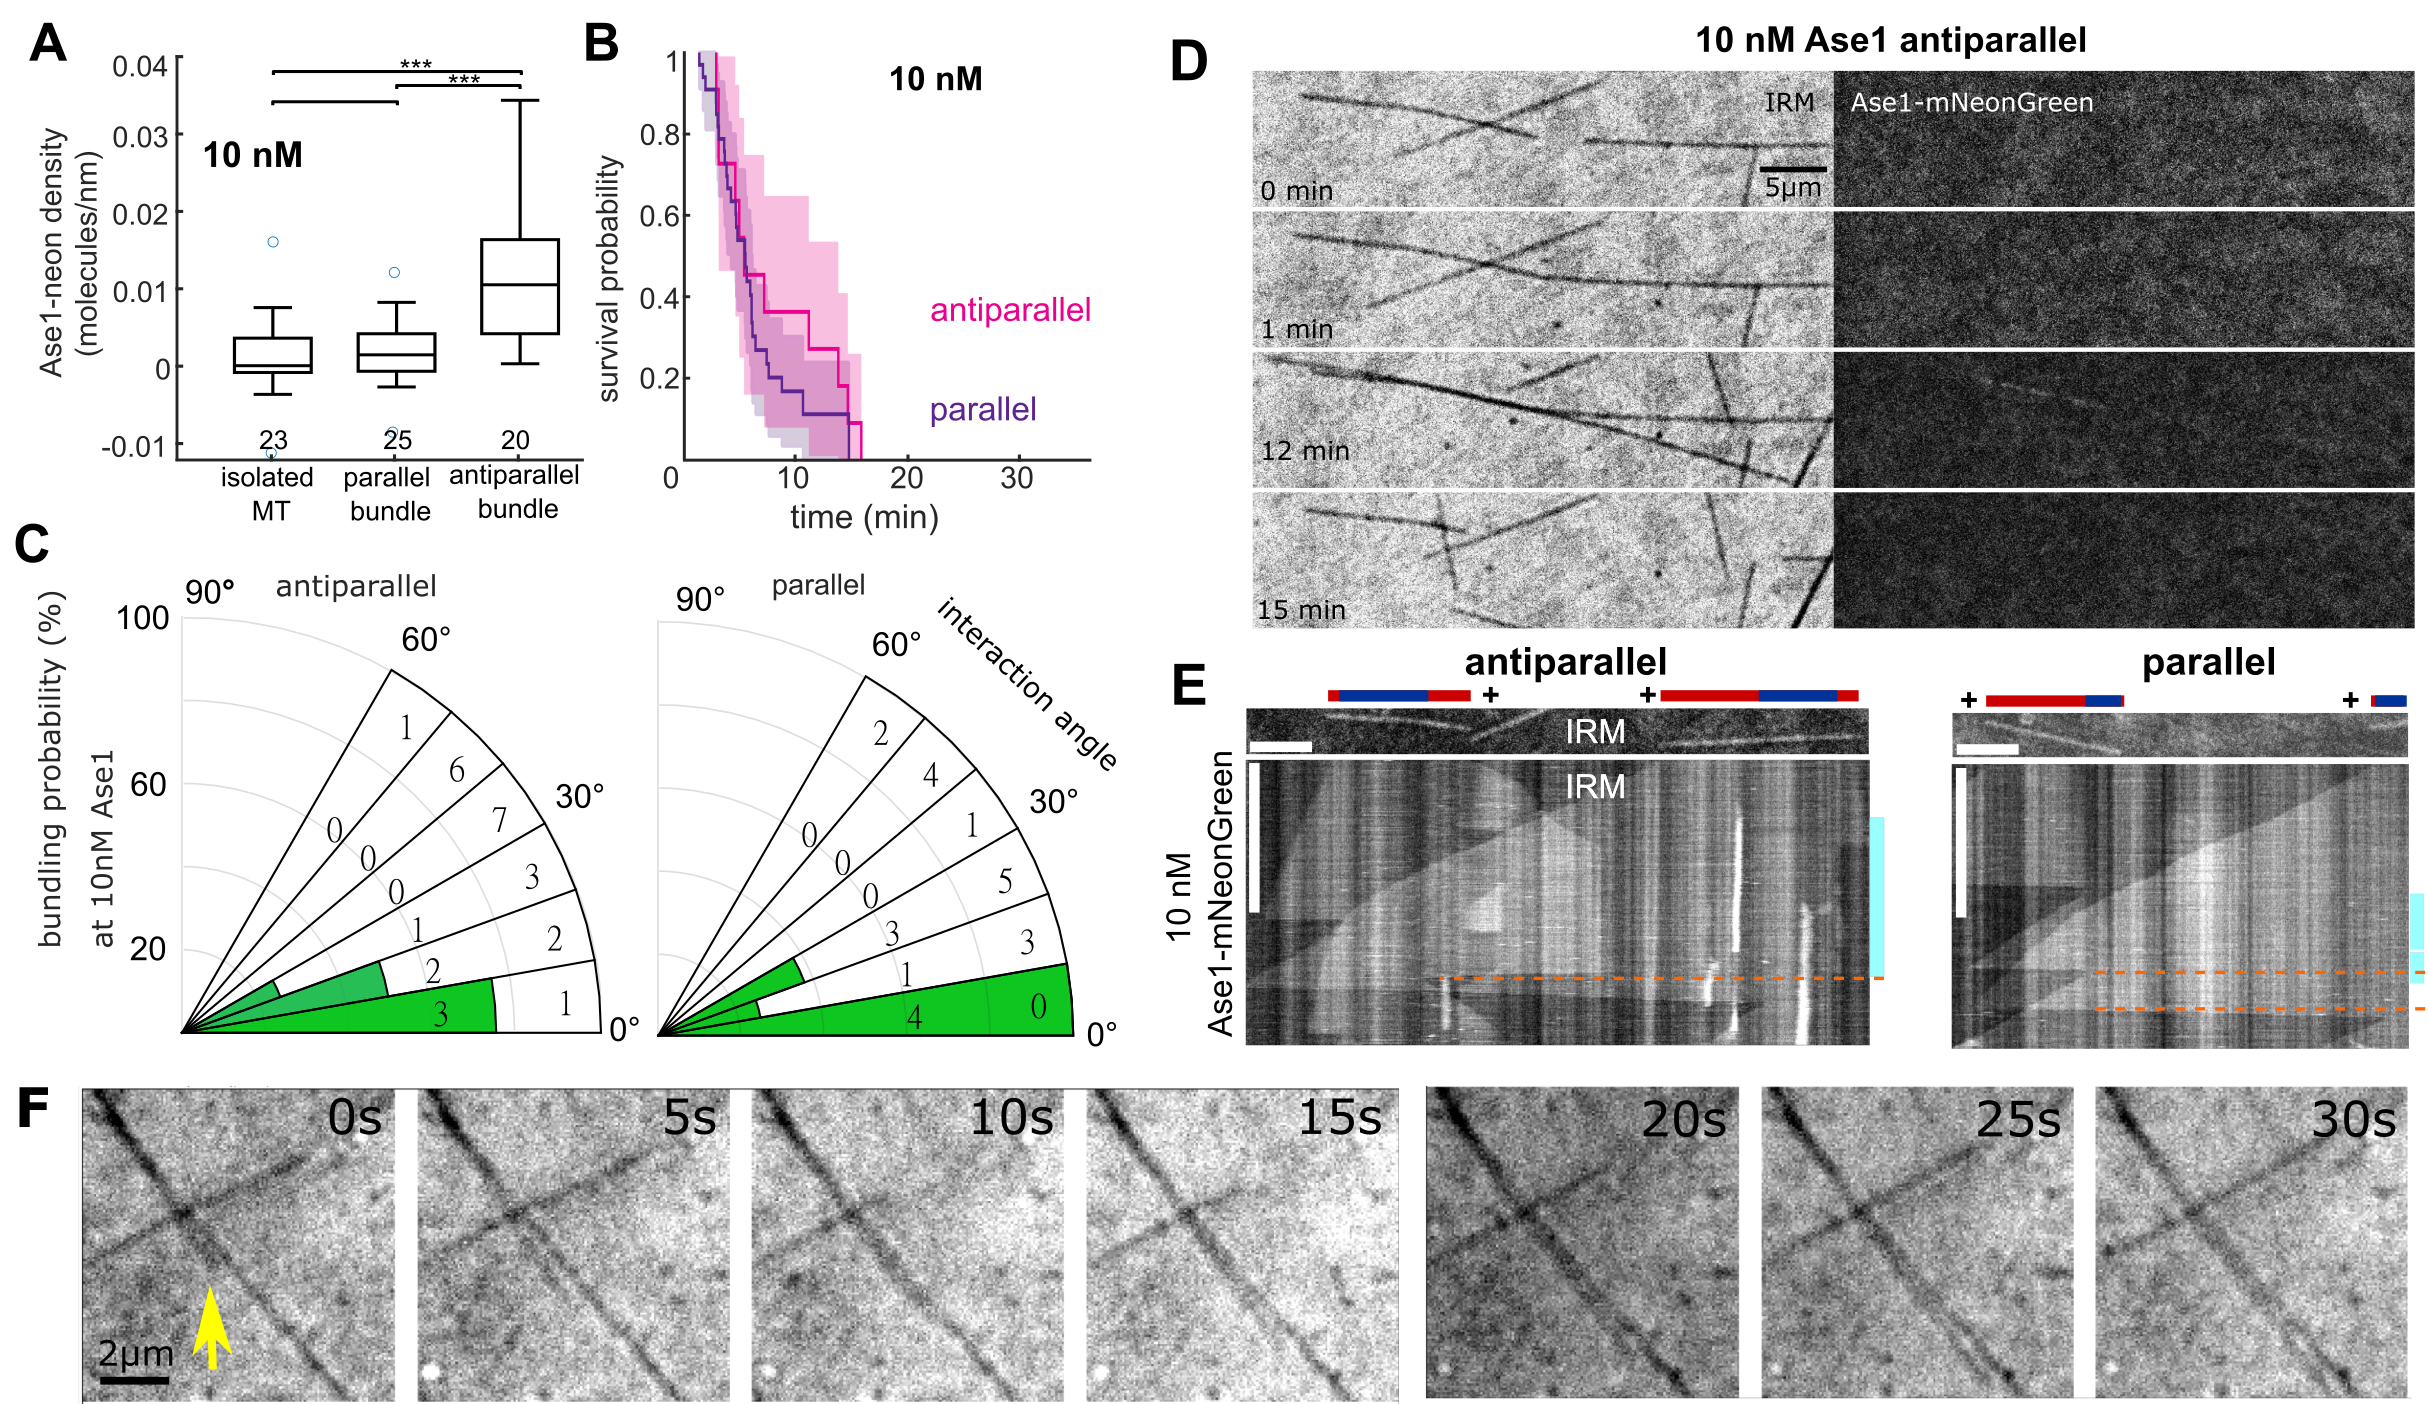
\includegraphics[width=1\linewidth]{Figures/ase1_1c.png}
    \caption[Antiparallel overlaps are not significantly stabilized at low Ase1 concentrations.]{
        (A,B) Quantifications of Ase1 densities and lifetimes for the 10nM Ase1 condition analogous to panels in \autoref{ase1b}. (C) Quantifications of bundling probabilities for the 10nM Ase1 condition analogous to \autoref{ase1a}D. (D) Snapshots of an antiparallel overlap at 10nM Ase1. (E) Kymographs for the 10nM Ase1 condition, representation analogous to \autoref{ase1a}A. The left panel shows the same event as D. (F) A microtubule polymerizing close to another, parallel microtubule at 0nM Ase1 (imaged with IRM). The tip of microtubule in question is indicated by a yellow arrow. As can be seen, no bundling is occurring despite the fact that the microtubules are very close to each other. Panels taken from \cite{Krattenmacher2024}.
        }\label{ase1c}
\end{figure}

Indeed, as indicated by the kymographs shown in \pref{ase1d}{A}, we found rescue frequencies to be increased for antiparallelly crosslinked microtubules at the Ase1 concentrations where we had observed increased lifetimes of these overlaps \pref{ase1d}{B}. To test whether Ase1 crosslinking might have other significant effects on MT polymerization, we next quantified the other three parameters of microtubule dynamic instability. We found that catastrophe frequencies were similar across the tested conditions, with no statistically significant difference between the different populations \pref{ase1d}{C}. Polymerization velocities were similar for all microtubule types, either isolated or bundled, across all tested Ase1 concentrations as well \pref{ase1d}{D}. However, at 420nM Ase1, MTs depolymerized markedly slower than at lower Ase1 concentrations. Further, at 42nM and 420nM Ase1, antiparallel MTs displayed a marked decrease in depolymerization velocity compared to isolated and parallel MTs \pref{ase1d}{E}. Thus, we observed Ase1 to only have a measurable effect on MT depolymerization, by reducing the rate of depolymerization and increasing chances for rescue, with no effect on polymerization.\par

If one only considers our results at 42nM, one could speculate that the particularly pronounced stabilization of antiparallel microtubules was due to the increased number of Ase1 molecules on antiparallel MTs as compared to parallel and isolated MTs. However, at 420nM, the number of Ase1 molecules per MT was similar across all types of MTs, while the antiparallel MTs still were more stable, despite indistinguishable Ase1 densities on antiparallel versus parallel MT overlaps \pref{ase1d}{F,G}. Thus, Ase1 engaged in antiparallel crosslinking seems to have a stronger effect on MT depolymerization than Ase1 engaged in parallel crosslinking or Ase1 not engaged in crosslinking. This deduction is supported by the fact that the number of Ase1 molecules engaged in Ase1 crosslinking was the only factor we could identify as influencing the frequency of rescues (note, however, that the number of molecules directly participating in the crosslinking process, i.e. simultaneously bound to both crosslinked microtubules, is not measurable in this assay). Notably, we with a different set of experiments ("Set B experiments," see \autoref{methods}) found the same result \autoref{ase1e}, showing the robustness of this finding: At these conditions, we observed antiparallely linked microtubules to exhibit rescues, at a density of around 0.2 molecules per nm which we at these buffer conditions had established with 1nM Ase1 \pref{ase1e}{B,C} (as a side note, the Ase1 used in these experiments was a slightly different construct, see \autoref{methods}). At these buffer conditions, isolated microtubules did not exhibit any rescues at all, even when we increased the Ase1 concentration from 1 to 6nM such that the Ase1 density on isolated microtubules was comparable to the Ase1 density on antiparallel bundles at 1nM Ase1 \pref{ase1e}{B,C}. The depolymerization velocity similarly decreased with increasing Ase1 concentration \pref{ase1e}{D}. Altogether, these results show that Ase1 can stabilize antiparallel microtubules while only having minor stabilization effects on MTs outside of such overlaps.

\begin{figure}[h]
    \centering
    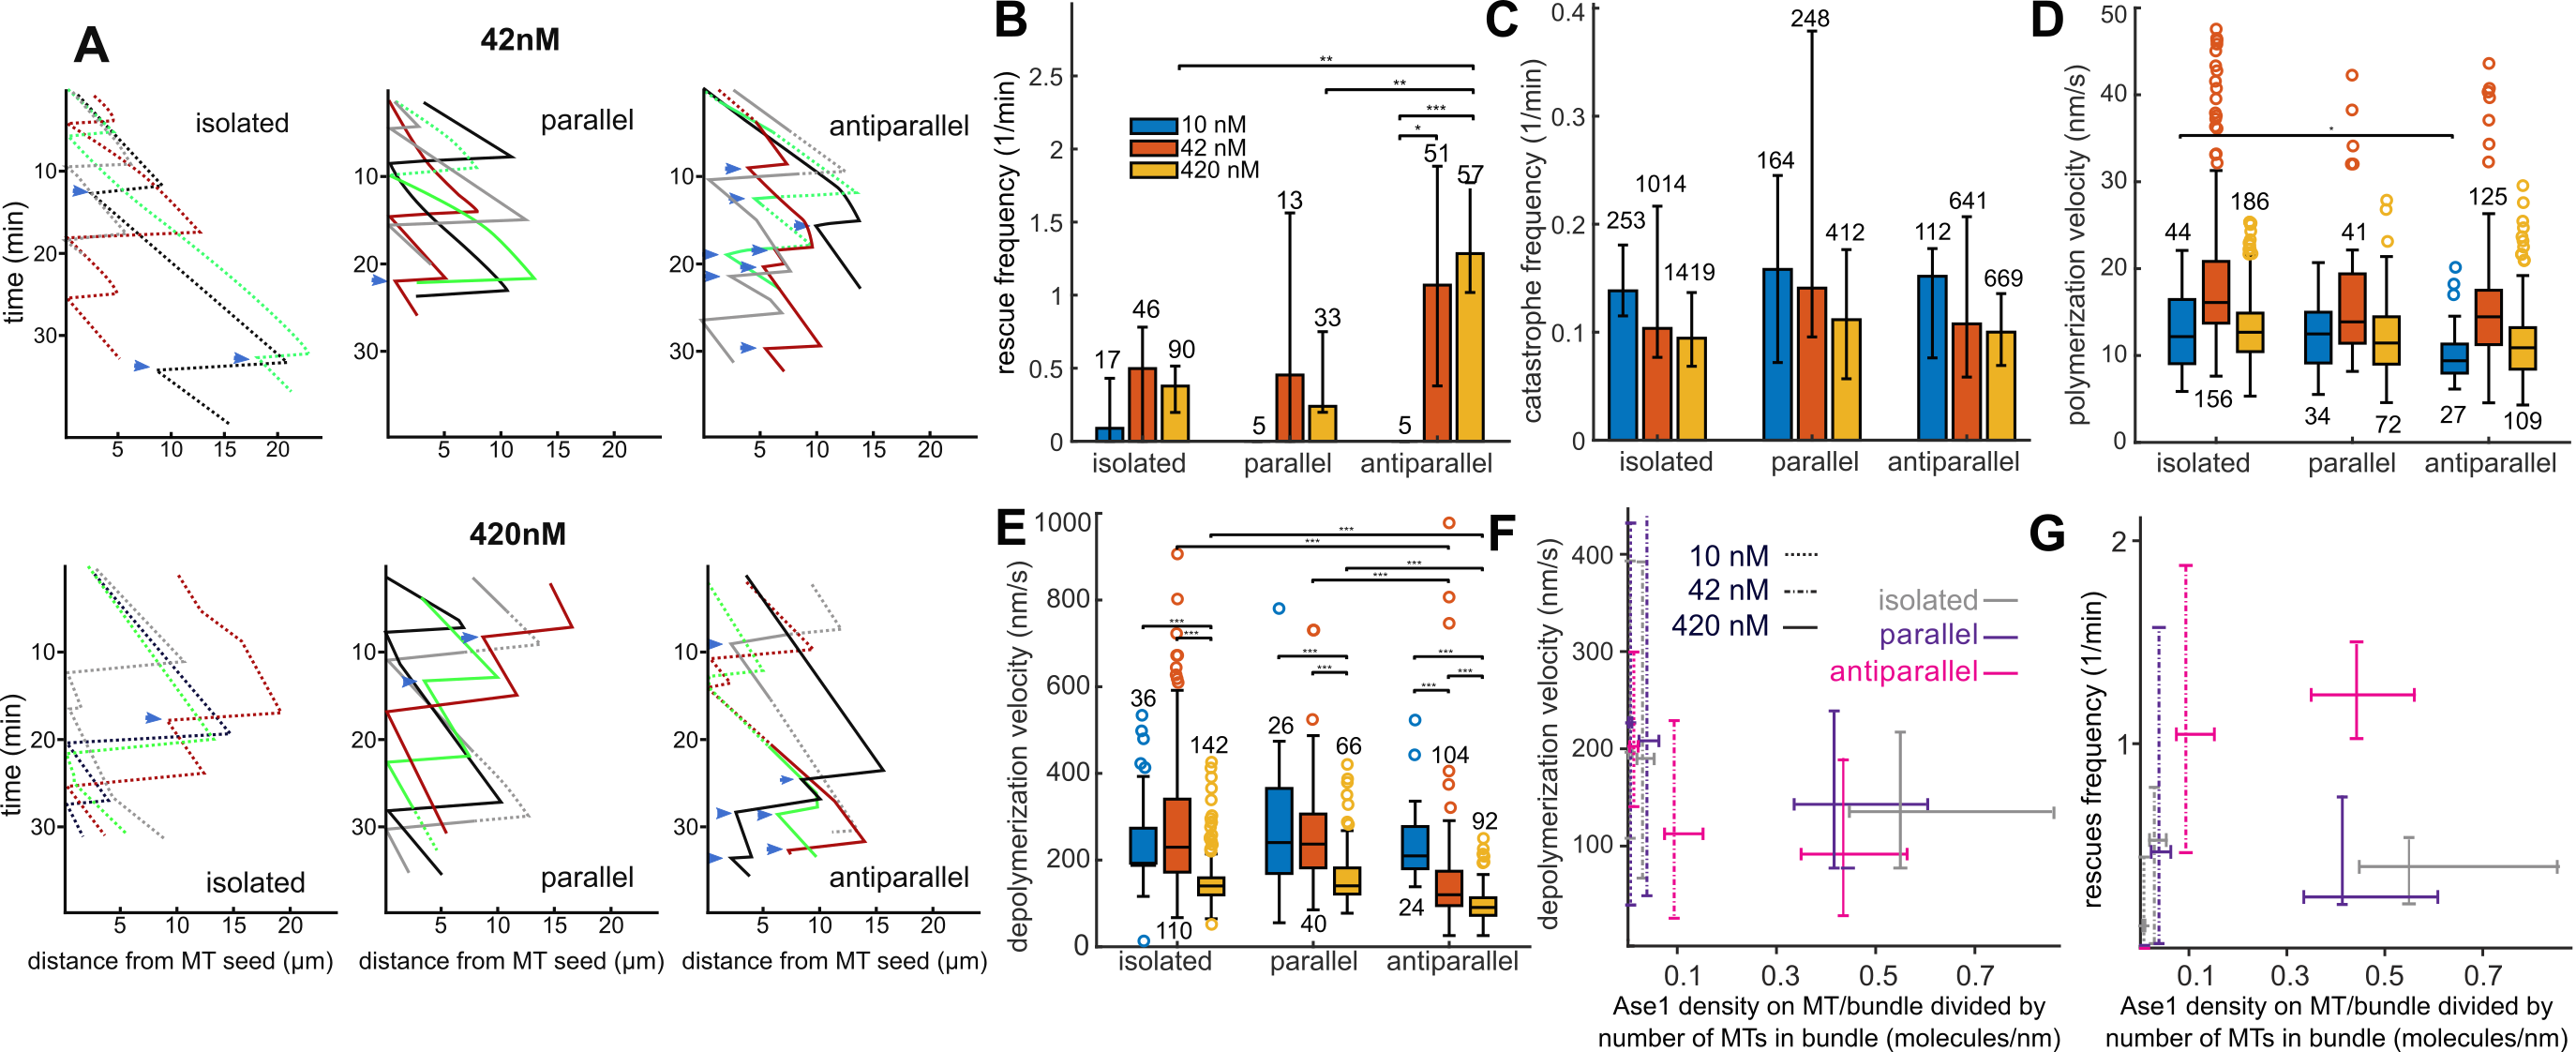
\includegraphics[width=1\linewidth]{Figures/ase1_1d.png}
    \caption[Representative kymograph traces.]{
    (A) Representative kymograph traces of the types of events we observed in our dataset which we present in \autoref{ase1a}, \autoref{ase1b} and \autoref{ase1c}A-E. Blue arrows indicate rescue events. Dotted lines indicate stretches where the MT was isolated. (B) Rescue frequency, (C) catastrophe frequency, (D) polymerization velocity, and (E) depolymerization velocity of dynamic MT plus ends in different configurations and in the presence of varying concentrations of Ase1-mNeonGreen. (F) Depolymerization velocity (see E) versus Ase1-mNeonGreen density on a given MT or bundle divided by number of MTs in that bundle (i.e., the density as shown in \autoref{ase1b}B is divided by 2 in the case of parallel and antiparallel MTs).  (G) Rescue frequency (see B) versus Ase1-mNeonGreen density (see \autoref{ase1b}B). All plots show results for the same experiments as shown in \autoref{ase1a} and \autoref{ase1b}. * p<0.05, ** p<0.01, *** p<0.001 (Tukey's test; only significance levels are visualized that share either the same MT type or the same concentration. No visual link between two populations sharing one such characteristic signifies  p>0.05. In B and C a given population comprises the frequencies recorded for the respective experiments, in D and E the velocities recorded for respective sampled periods). Boxplots are weighted by the length of a sampled period of polymerization or depolymerization. In boxplots, the numbers indicate the number of recorded events, in bar plots, the numbers indicate the sum of the length of all sampled periods of polymerization or depolymerization (in minutes). In bar plots, the height of the bar indicates the catastrophe/rescue frequency as determined from all time lapses (number of total events divided by total duration of depolymerization), while the error bars indicate the lowest and highest rates as determined from each isolated time lapse; velocities are normalized to the median velocity of isolated MTs (Methods). Panels taken from \cite{Krattenmacher2024}.
        }\label{ase1d}
\end{figure}

\begin{figure}[h]
    \centering
    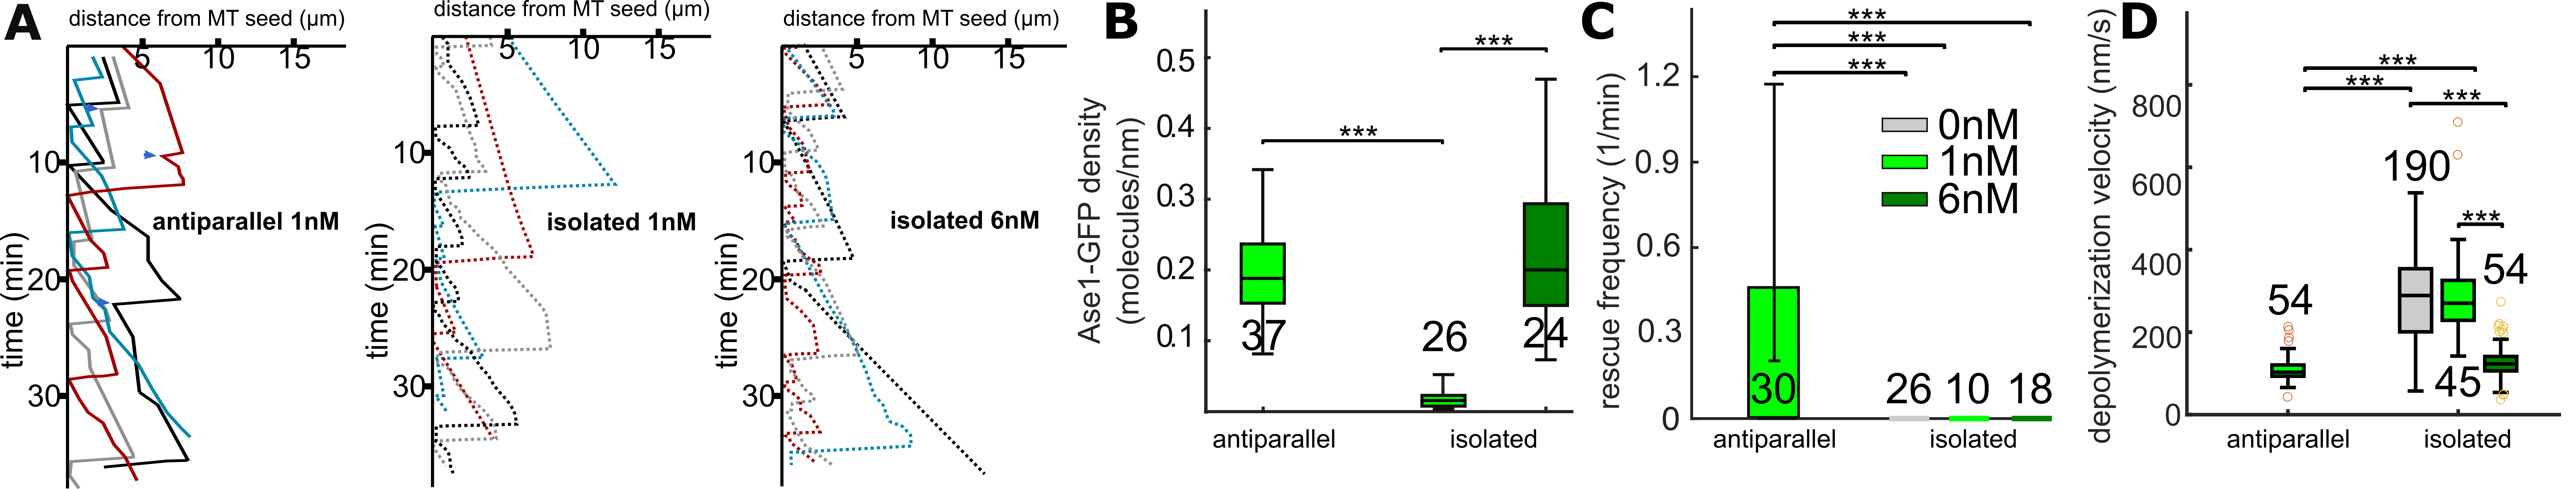
\includegraphics[width=1\linewidth]{Figures/ase1_1e.png}
    \caption[Set B experiments microtubule dynamics.]{
    Data obtained from a second set of experiments ("Set B experiments", see \autoref{methods}) with different experimental parameters than the data from the set of experiments shown thus far ("Set A experiments"). (A) Representative kymograph traces, representation analogous to \aref{ase1d}{A}. (B) Quantification of the density of Ase1-GFP(Methods). The numbers below the boxes denote the number of analyzed microtubule bundles. (C) Rescue frequency and (D) depolymerization velocity, representations analogous to \aref{ase1d}{B,E}. Legend for B-D in C, showing the concentration of Ase1-GFP in each set of experiments. Panels taken from \cite{Krattenmacher2024}, except panels C and D, which were created only for this thesis.
        }\label{ase1e}
\end{figure}

\FloatBarrier
\subsection{Interactions between Ase1 and the depolymerizing microtubule end}
\begin{figure}[h]
    \centering
    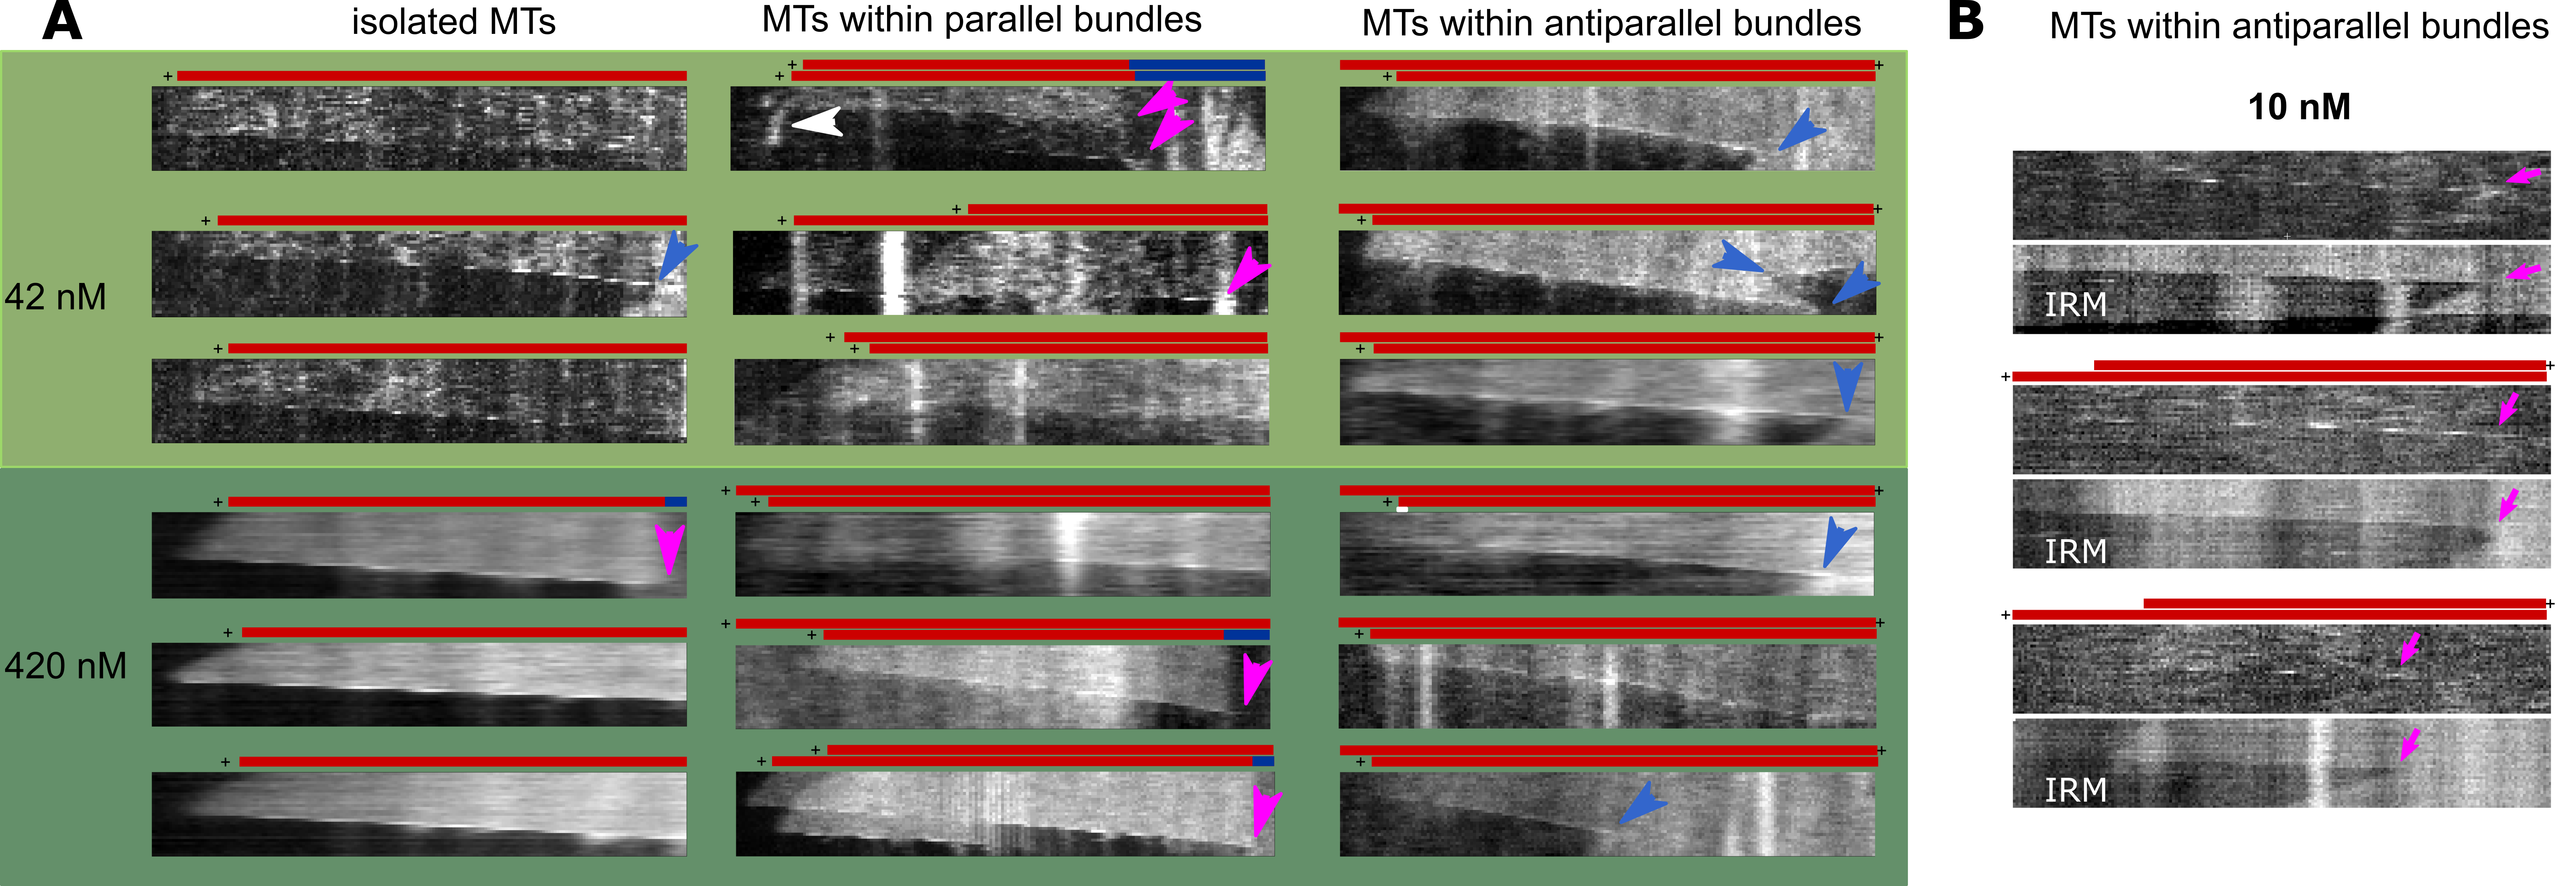
\includegraphics[width=1\linewidth]{Figures/ase2a.png}
    \caption[Set A experiments kymographs showing Ase1 herding.]{Kymographs of depolymerization events (Set A experiments as shown in \aref{ase1d}{A}). (A) Kymographs of all examined microtubule configurations at 42nM and 420nM Ase1. (B) Kymographs of events observed at 10nM Ase1 (antiparallel overlaps only since at this concentration there was no Ase1-mNeonGreen signal at the ends of parallel overlaps and isolated MTs). Each kymograph is 12 µm in width and 150 seconds in height, contrast and balance varies from panel to panel (each kymograph shows a different MT). To facilitate understanding of the kymographs, rescues are pointed out with blue arrows. Pink arrows indicate a MT tip reaching its GMPCPP seed. The white arrow indicates where one of the parallel MTs, before catastrophing, had briefly engaged in antiparallel crosslinking with another isolated MT. Where no arrows are shown, the MT continues to depolymerize toward the right. Panels taken from \cite{Krattenmacher2024}.
        }\label{ase2a}
\end{figure}
Given that we had shown that Ase1 can stabilize depolymerizing microtubules, we suspected that Ase1 molecules very likely interact directly with depolymerizing MT ends. This is indeed what we found when examining the distribution of Ase1. While Ase1 did show no preference for binding to polymerizing MT ends, the kymographs which we had generated showed that Ase1 accumulated at depolymerizing MT ends, for Set A experiments \pref{ase2a}{A,B} as well as Set B experiments \pref{ase2b}{A}. We now set out to quantify this effect. Because the data for Set B experiments allowed for a more fine-grained analysis due to a higher framerate and a more pronounced accumulation effect, we in the following limited our analysis to the Set B experimental data. Given that isolated and parallel MTs behaved very similarly in our assays (though only in Set A experiments we observed a sufficiently high number of parallel overlaps for a thorough analysis), we also chose to focus on comparing isolated and antiparallel MTs.\par
\begin{figure}[h]
    \centering
    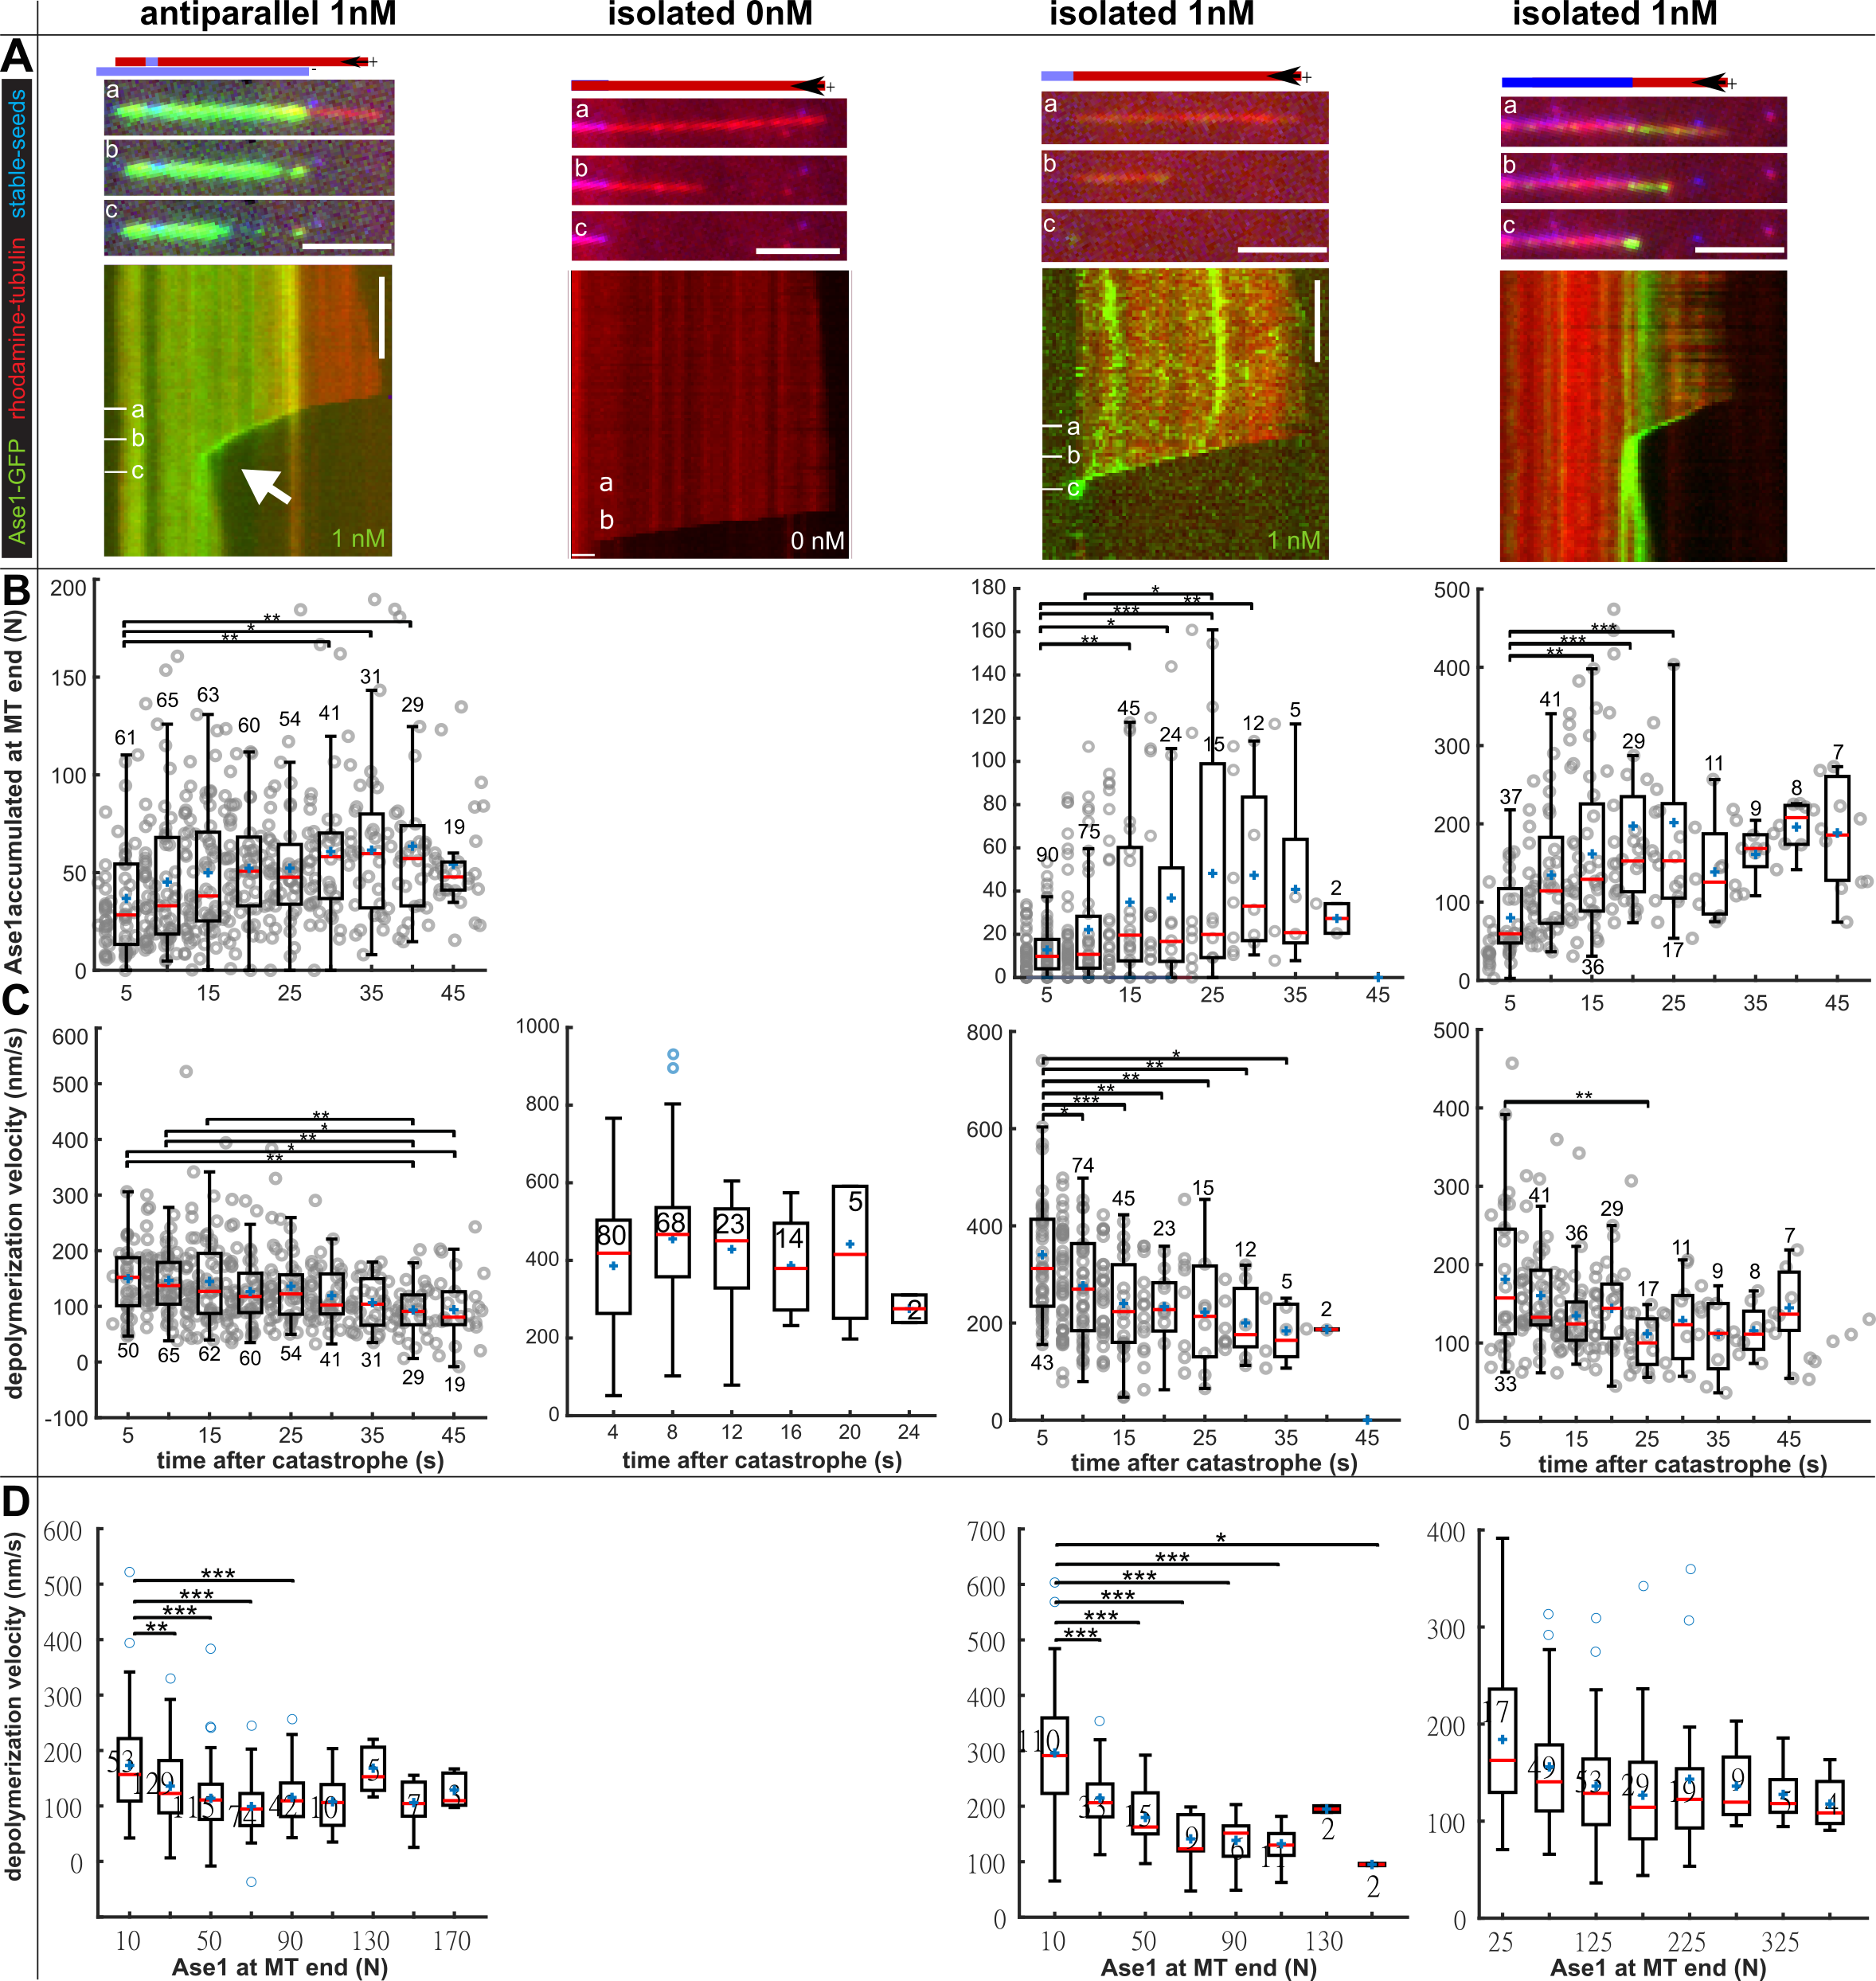
\includegraphics[width=1\linewidth]{Figures/ase2b.png}
    \caption[Ase1 accumulates at depolymerizing MT ends.]{Experimental data on herding of Ase1 (Set B experiments as shown in \aref{ase1e}{A}). (A) Kymographs of depolymerizing MTs. The stabilized GMPCPP-MT seeds were labelled with 15\% rhodamine and 15\% Alexa647 (or, alternatively, with 2\% Alexa647), while the free tubulin in solution was labelled with 7\% rhodamine. In sketches, dynamic extensions with GDP lattices are colored red, and stabilized GMPCPP seeds are colored blue or light blue (in case of the weakly-labelled seeds). The scale bars are 5 micron and 1 minute, contrast and balance vary from panel to panel (each kymograph shows a different MT). White arrows highlight rescue events. (B) The number of additional Ase1 molecules at the end of depolymerizing MTs, plotted over the time passed since the catastrophe. Each data point represents data extracted from one line scan. (C) The frame-to-frame depolymerization velocity of MTs over time (analogous to B). Because the exact time of catastrophe is unknown due to limits in temporal resolution, the velocity measurement right after catastrophe underestimates the actual velocity. (D) Instantaneous depolymerization velocity plotted over number of additional Ase1 molecules at the MT end. Panels taken from \cite{Krattenmacher2024}.
        }\label{ase2b}
\end{figure}

Our quantitative analysis of Ase1 accumulation at depolymerizing microtubule ends confirmed the visual impression given by the kymographs - Ase1 was indeed accumulating at depolymerizing MT ends, for both isolated and antiparallel MTs \pref{ase2b}{B}. In addition, the quantitative analysis also revealed that the Ase1 accumulates were growing the quickest during the early stages of depolymerization \pref{ase2b}{B}. Intuitively, one may expect that this accumulation is related to the stabilization of microtubules during depolymerization. Indeed, Ase1 accumulation correlated with a decrease in depolymerization speed \pref{ase2b}{B-D}. While this correlation does not imply a causal relationship, it does lend support to the existence of such a relationship. An alternative explanation could be a possible hidden third factor, most notably the natural slowdown of depolymerization velocity after catastrophe which has been observed by others \parencite{Luchniak2023}. In other words, it is conceivable that depolymerizing MTs accumulate Ase1 and slow down over time, and that these two phenomena are not causally related. However, in the absence of Ase1 we had not observed any slowdown in MT depolymerization comparable to what we observed in the presence of Ase1 \pref{ase2b}{C}. \par

\begin{figure}[h]
    \centering
    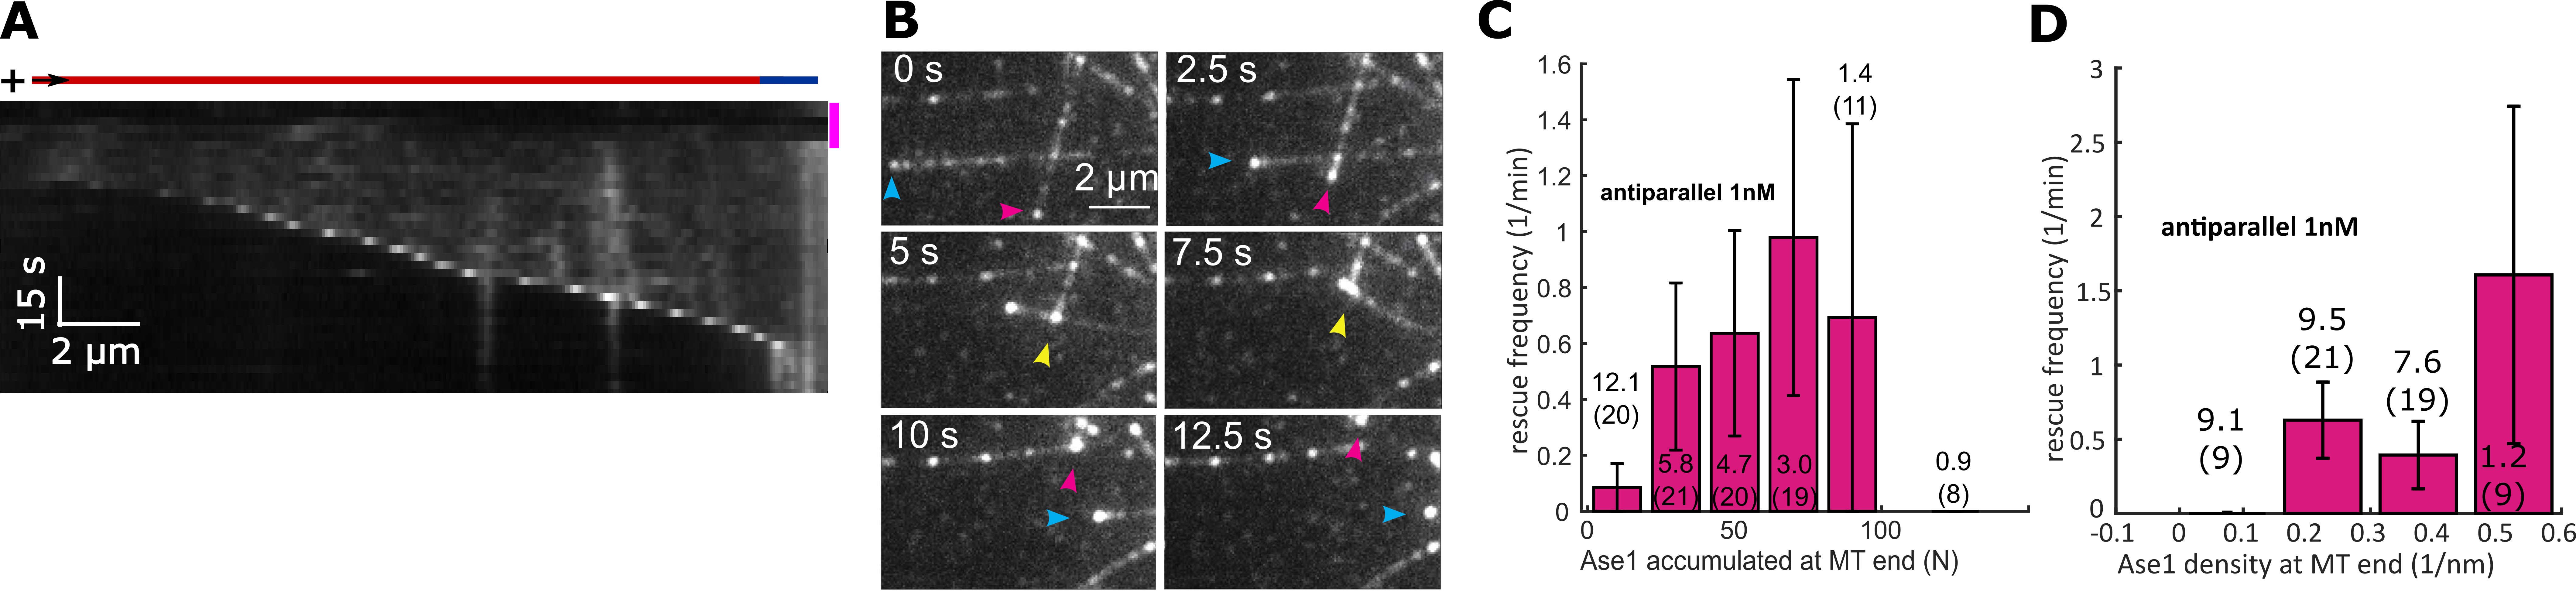
\includegraphics[width=1\linewidth]{Figures/ase2c.png}
    \caption[Ase1 is herded by depolymerizing MTs.]{
    (A) Kymograph (Ase1-mNeonGreen channel) of depolymerizing MT. In this experiment, Ase1 and tubulin had been removed from the assay buffer during the time frame indicated by the pink bar next to the kymograph, prompting subsequent MT depolymerization and concomitant Ase1 accumulation at the end. (B) Time series of micrographs (Ase1-GFP channel) showing an event where the accumulated Ase1 at one depolymerizing MT end (indicated by red arrows) causes the end to “drag” a MT it crosses with it, thereby bending it (yellow arrows). The blue arrows indicate the (depolymerizing) end of the MT before and after it got bent. (C) Rescue frequency plotted over number of additional Ase1 molecules at the MT end. The duration depolymerized at a respective x-value was added to the respective bin. The number of rescues observed in the same bin (N) was then divided by the sum of depolymerization durations (shown in min, the number in parentheses refers to the number of MTs) to estimate the rescue frequency. The correlation coefficient (weighted \parencite{Pelletier2024} by sums of depolymerization durations) is 0.67. The total length of a given error bar equals two times the square root of the number of the rescues in the corresponding bin divided by the sum of the time depolymerized in the corresponding bin. (D) Rescue frequency plotted over the height of the peak of the Ase1 density at the MT end (the weighted correlation coefficient is 0.76). Representation analogous to C. C and D show data from Set B experiments. Panels taken from \cite{Krattenmacher2024}.
        }\label{ase2c}
\end{figure}

Our findings so far suggested that we observed "herding" of Ase1 by the depolymerizing MT end, a phenomenon which has recently been reported for a synthetic MT crosslinker \parencite{Drechsler2019}. To confirm this, we needed to exclude the possibility that Ase1 specifically tracks depolymerizing MT ends by having a higher affinity for depolymerizing MT regions. We thus performed an experiment where we removed both Ase1 and tubulin from solution after first having polymerized Ase1-decorated MTs. We found Ase1 to still accumulate at the ends of depolymerizing MT \pref{ase2c}{A}, indicating that the accumulates are indeed comprised of Ase1 molecules that were already bound to the MT lattice before catastrophe had occurred. As reported for the synthetic polymer \parencite{Drechsler2019}, we also observed instances of depolymerizing MT ends which herded Ase1 molecules pulling on other MTs \pref{ase2c}{B}. This indicates that substantial forces can be transmitted via Ase1 herding.\par

What is the impact of Ase1 herding on microtubule depolymerization for isolated versus antiparallel MTs? Again, we found that the impact of single Ase1 molecules on the depolymerization of antiparallel MTs is stronger than in the case of isolated microtubules: While isolated microtubules at 6nM Ase1 herded more Ase1 than antiparallel microtubules at 1nM Ase1, they did not depolymerize more slowly than antiparallel MTs \pref{ase2b}{B,C}. For antiparallel MTs, we also observed the number of herded Ase1 molecules to positively correlate with the probability of a rescue occuring \pref{ase1c}{C} (a phenomenon we could not test for isolated MTs since they did not exhibit any rescues in this dataset; furthermore, the rescue frequency of isolated MTs appears independent from Ase1 density, see \aref{ase1d}{B}). Moreover, the Ase1 density at the microtubule end, which is a measure for not only accumulated Ase1 but the total number of Ase1 molecules present at the end, also shows a positive correlation with rescue frequency \pref{ase1c}{D}.\par
 
Our experiments thus demonstrate that lattice-bound Ase1 molecules are herded by the depolymerizing MT ends and that the number of swept Ase1 molecules correlates with reduced depolymerization velocity, and, for antiparallel overlaps, with an increased probability of rescue. 


Within a few hundred nanometers at the depolymerizing ends of antiparallel overlaps and isolated MTs, we observed accumulation of Ase1 molecules (Figure 3A,B, Figure S3D).